\documentclass[../../main.tex]{subfiles}

%-----------------------------------------------------------%

\begin{document}

% \begin{equation}
%     \boxed{ \color{blue}    \color{black}}
% \end{equation}

%-----------------------------------------------------------%

% -------- %
% Overview %
% -------- %

\subsubsection{Overview} % Summary
The version 2 Model for \SIS involves -
\begin{enumerate}[label={}]
    \descitem{Optics Model -} The Optics Model in Version 2 is the simplest possible system, involving straight line ray optics. This takes no aberrations into account. 
    \descitem{CMOS Model -} The CMOS Model takes Sensor Specifications into account, along with the major Sensor Noises. (The sensor specifications are taken from the datasheet of PYTHON-1300, which is the sensor of choice at the present. 
\end{enumerate}

A modest flowchart of the Sensor Model is as follows:

\begin{Flowchart}[h!]
    \centering
    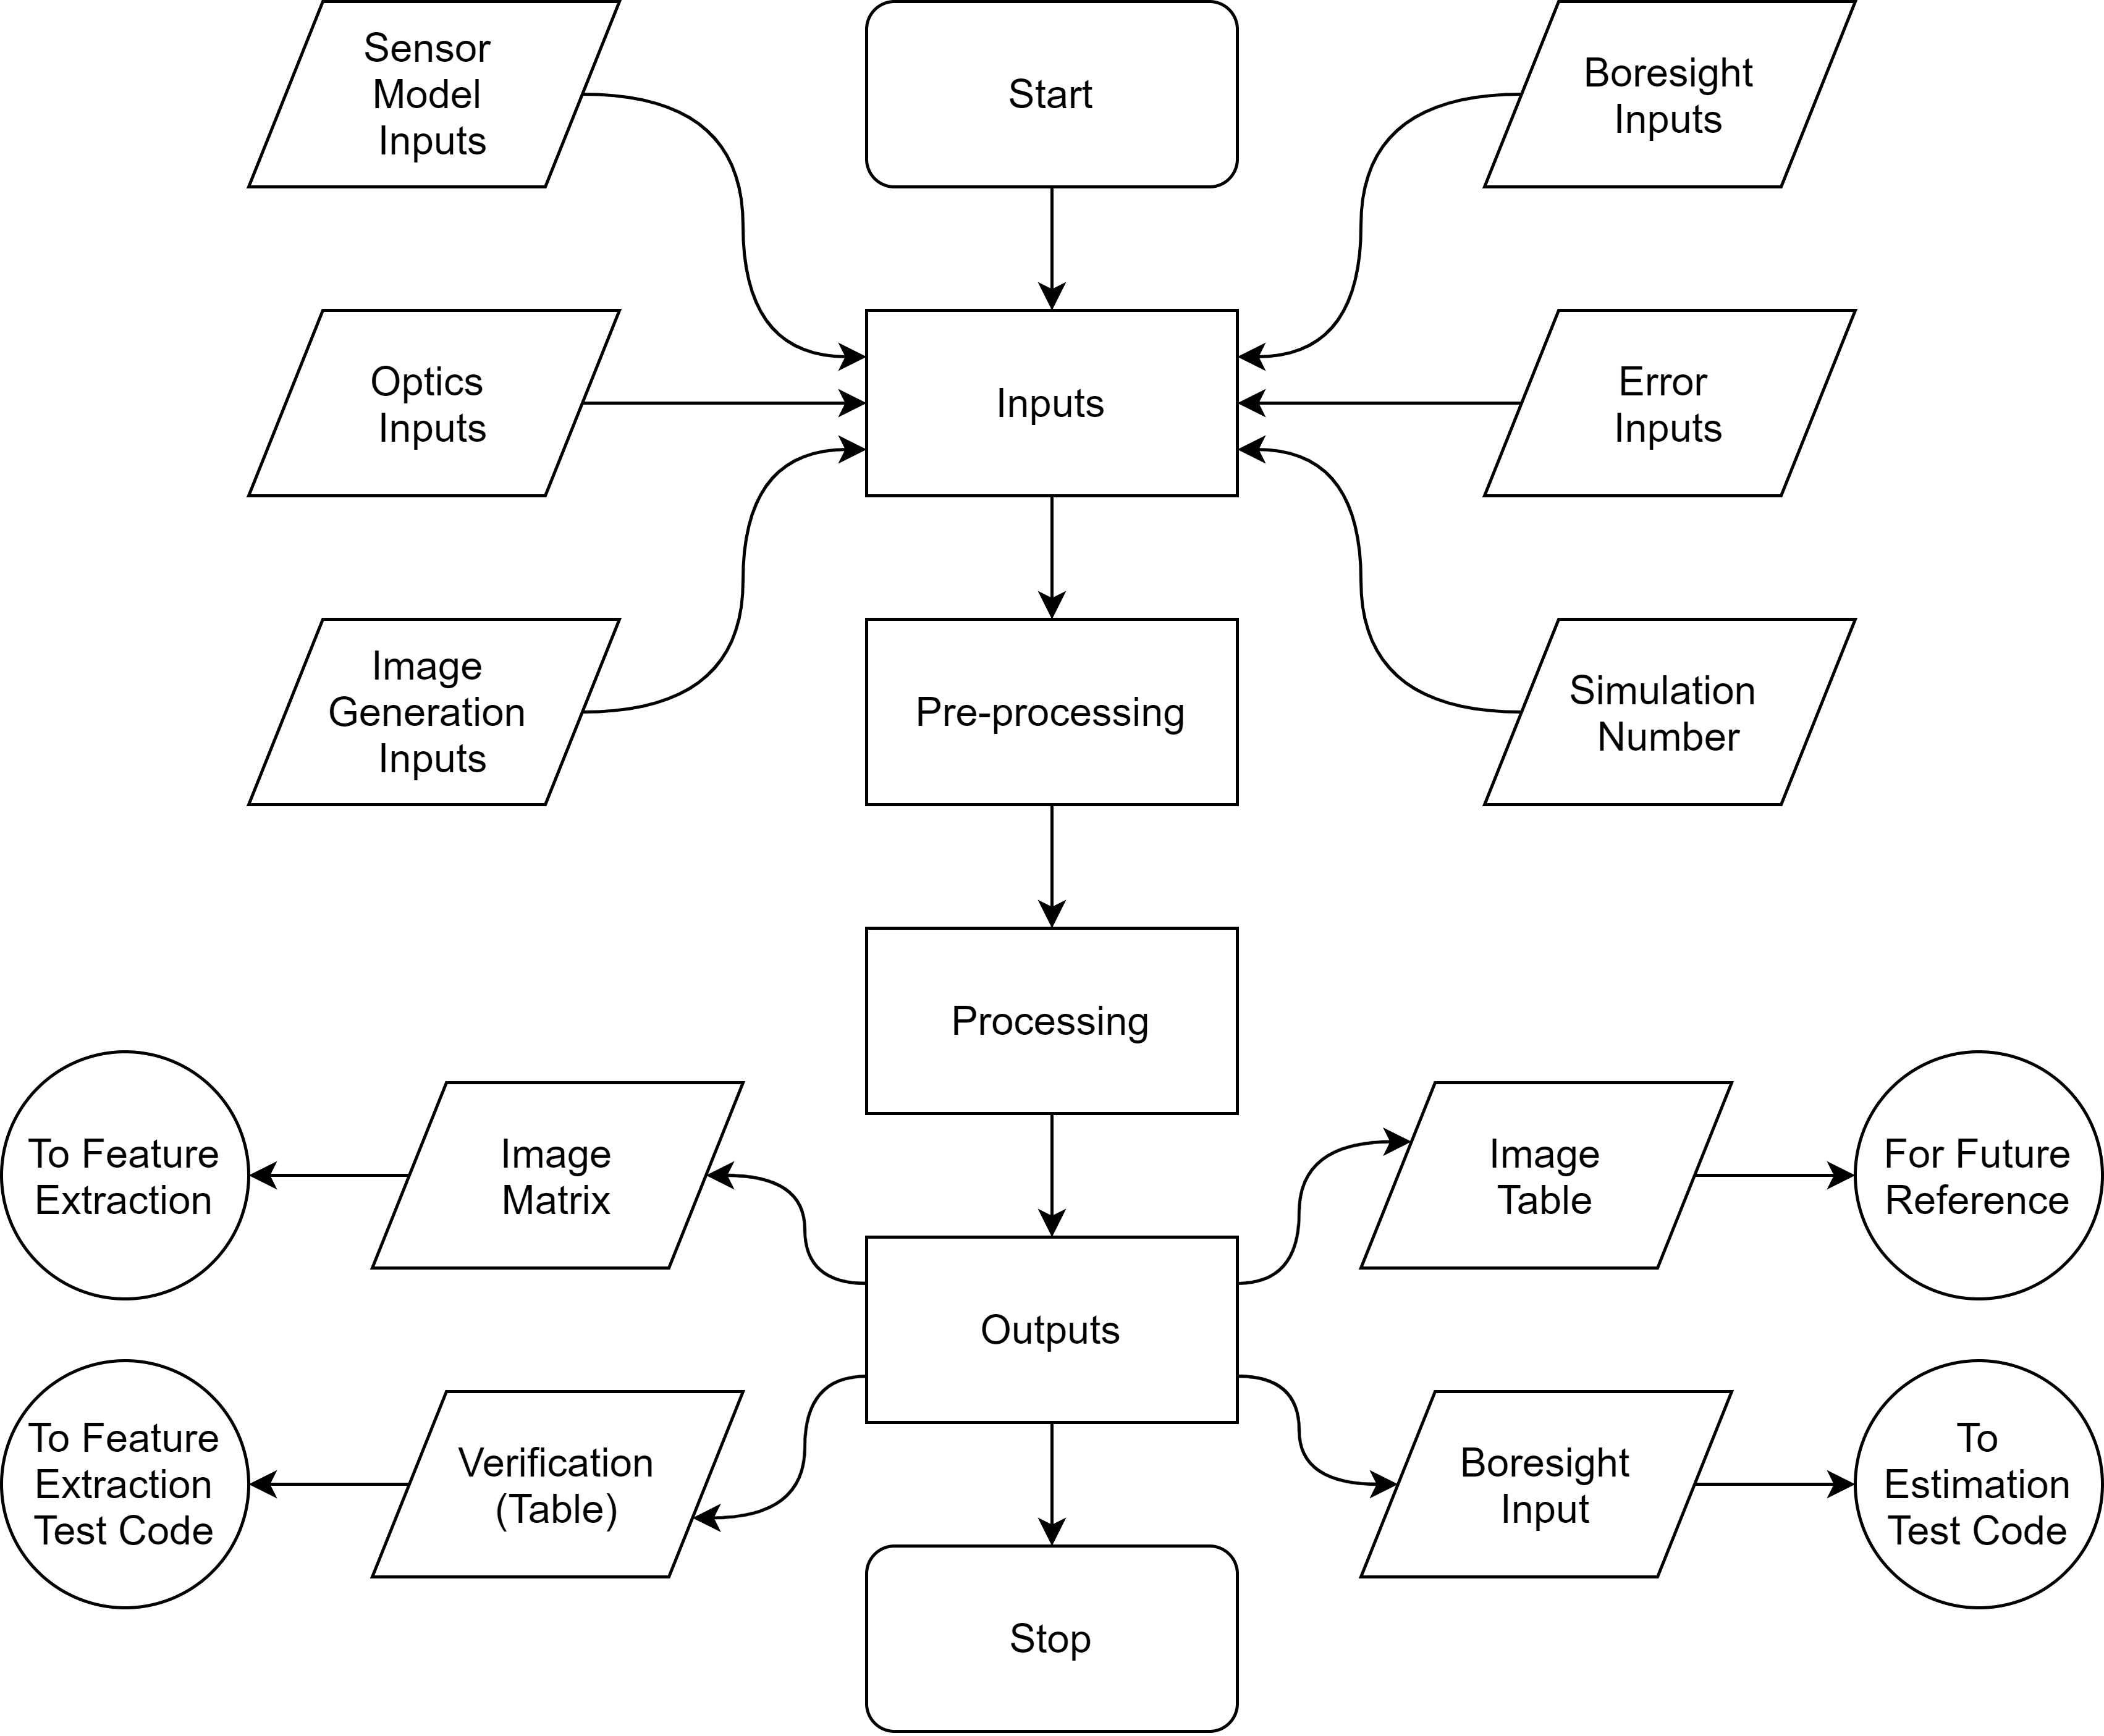
\includegraphics[width=\textwidth]{Figures/Model/Sensor Model v2.png}
    \caption{Star Image Simulation Flowchart - Version 2}
    \label{fig:SIS_v2}
\end{Flowchart}

% ------ %
% Inputs %
% ------ %
\newpage
\subsubsection{Inputs}
The inputs to the \SISM are as follows:
\begin{enumerate}[label={}]
    \descitem{Star Catalogue -} This is the SSP Star Catalogue, which is pre-processed for \SIS. The SSP Star Catalogue has been generated from the SKY 2000 Catalogue. 
    \descitem{Boresight Inputs -} This includes the Boresight data, or the Attitude data at instants when images are to be generated. This is currently manually created, however, in the future, this is the ouput of the Dynamics Block.
    \descitem{Sensor Model Inputs -} This includes global inputs to the \SISM, which includes parameters like Star Magnitude Limit for \SISM and the Number of Boresight Inputs. 
    \descitem{Optics Inputs -} This includes parameter inputs from Optics Perspective, i.e. relates to the Lens System and the CMOS Sensor.
    \descitem{Image Generation Inputs -} This includes parameters related to Image Generation at the CMOS Sensor taken from the data-sheet for PYTHON-1300.
    \descitem{Error Inputs -} This includes all the parameters required to model the Sensor Noise. These have been taken from the data-sheet for PYTHON-1300.
\end{enumerate}

% -------------- %
% Pre-Processing %
% -------------- %

\subsubsection{Pre-processing} % 2 parts - Loading constants, and Pre-processing of Catalogue
The pre-processing sub-block involves 2 steps -
\begin{enumerate}[label={}]
    \descitem{Loading Inputs and Calculating Parameters -} This sub-sub-block involves loading all the inputs from the .xlsx files, and calculations of parameters from the inputs, where the inputs are converted into SI units for uniformity and dependent parameters are calculated from the independent parameters. 
    \descitem{Pre-processing Catalogue -} The SSP Star Catalogue is pre-processed to include parameters which are used multiple times in the \SIS. These include the calculation of the Unit Vectors in the ICRS Frame from the Right Ascension, Declination values given in the SSP Star Catalogue. Unnecessary columns are also removed in this step. 
\end{enumerate}

A modest flowchart for the Pre-processing sub-block is given here -

\begin{Flowchart}[h!]
    \centering
    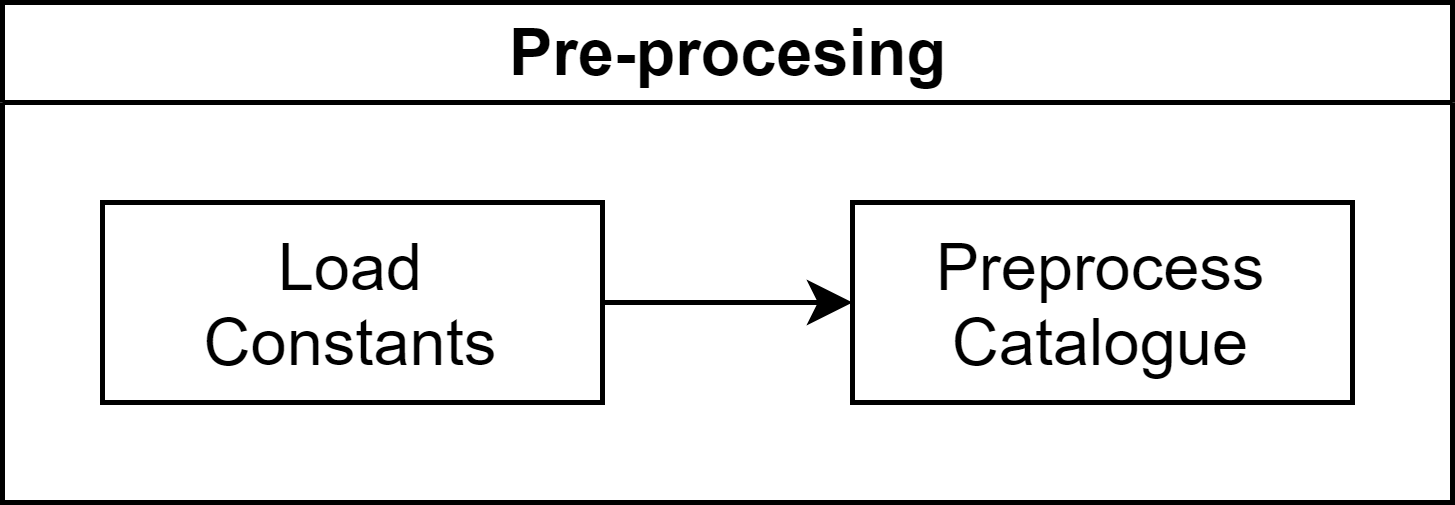
\includegraphics[scale=0.09]{Figures/Model/Pre-processing.png}
    \caption{Pre-Processing Sub-Block - Version 2}
    \label{fig:SIS_v2_PP}
\end{Flowchart}

% ---------- %
% Processing %
% ---------- %

\subsubsection{Processing}

The flowchart for the Processing sub-block is given in Figure \ref{fig:SIS_v2_PR}

\begin{Flowchart}[h!]
    \centering
    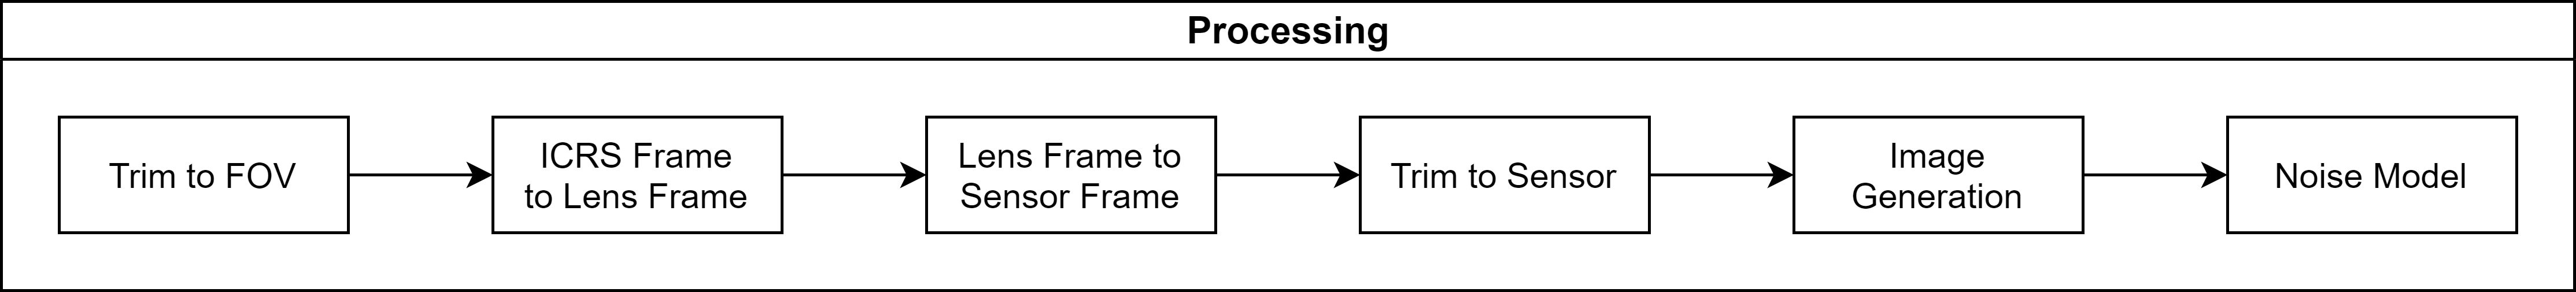
\includegraphics[scale=0.09]{Figures/Model/Processing.png}
    \caption{Processing Sub-Block - Version 2}
    \label{fig:SIS_v2_PR}
\end{Flowchart}

Visual information is recorded via the CMOS sensor placed at the focal plane of the optics system to measure the light gathered during the exposure. The sensor is platted into an array of pixels, each of which is tasked to gather the light arriving within a small patch of sensor area. The efficiency with which the sensor and its pixels gather light, and the accuracy to which it determines the amount gathered by each pixel, are crucial in determining the quality of the recorded image. \cite{DSLRs} Hence, we need to have an accurate model for the CMOS Sensor. The noise effects in the CMOS Sensor have been separated out into the Noise Model.

The processing sub-block involves the following steps -
\begin{enumerate}[label={}]
    \descitem{Trim to FOV -} This sub-sub-block trimming the database of all the stars to those within the Field of View of the Star Tracker, given its attitude. 
    \descitem{ICRS Frame to Lens Frame -} This sub-sub-block transforms the unit vectors of the stars in the database from the ICRS Frame to the Lens Frame (3D)
    \descitem{Lens Frame to Sensor Frame -} This sub-sub-block projects the 3D unit vectors of the stars onto the 2D Sensor Frame. 
    \descitem{Trim to Sensor -} This sub-sub-block trims the stars to within the Sensor Frame. This is because there can be stars within the Field of View, but still outside the Sensor Frame. 
    \descitem{Image Generation -} This sub-sub-block generates the image using the star database and the inputs. For more details, refer to \ref{subsubsection:IG}.
    \descitem{Noise Model -} This sub-sub-block adds the required noises at the Sensor.
\end{enumerate}

% ---------------- %
% Image Generation %
% ---------------- %

\subsubsection{Image Generation \label{subsubsection:IG}}
\blindtext


% ------------------- %
% CMOS Sensor - Intro %
% ------------------- %

\subsubsection{Introduction to CMOS Sensor}
CMOS image sensors with global shutter (GS) are becoming popular. It is possible to capture the shape of a high speed moving object with high accuracy without distortion. Conventional CMOS sensors adopt rolling shutter (RS) method. In the RS method, an exposure is sequentially performed for each row pixel and there is a slight time difference in signal readout for each row pixel. Thus, the high-speed moving object is distorted. For example, when a flash is used during shooting, the flash band phenomenon may occur with different brightness of the image on the top and the bottom. CMOS image sensor with GS exposes all the pixels at the same time and it can take a non-distorted photograph of the high speed moving object such as a rotating propeller. 

GS CMOS image sensor with small pixel is demanded for high resolution pictures and sensing. In practical use of GS sensor, it is important to achieve high signal-to-noise ratio. High quantum efficiency (QE) is required to increase the signal intensity. In order to increase the QE, it is necessary to provide more light to the photo diode (PD) even in small size pixel. In terms of noise, it is necessary to care the noise caused by GS structure.

% ----------- %
% Noise Model %
% ----------- %

\subsubsection{Noise Model} % Introduction to noise model
The incoming light from the stars is the signal we need the CMOS Imaging Sensor to transcribe faithfully; inaccuracies in the recording process constitute noise, and inhibit the ability to reconstruct the Star Vectors in the image frame, which leads to inaccuracies in the Star Tracking and Star Matching Algorithms. In order to extract the best performance from the CMOS Imaging Sensor, it is helpful to have an understanding of the various contributions to image noise and how various design choices in the Lens System and the choice of CMOS Sensor affect this noise.

A flowchart for the Noise Model for Version 2 is as follows -

\begin{Flowchart}[h!]
    \centering
    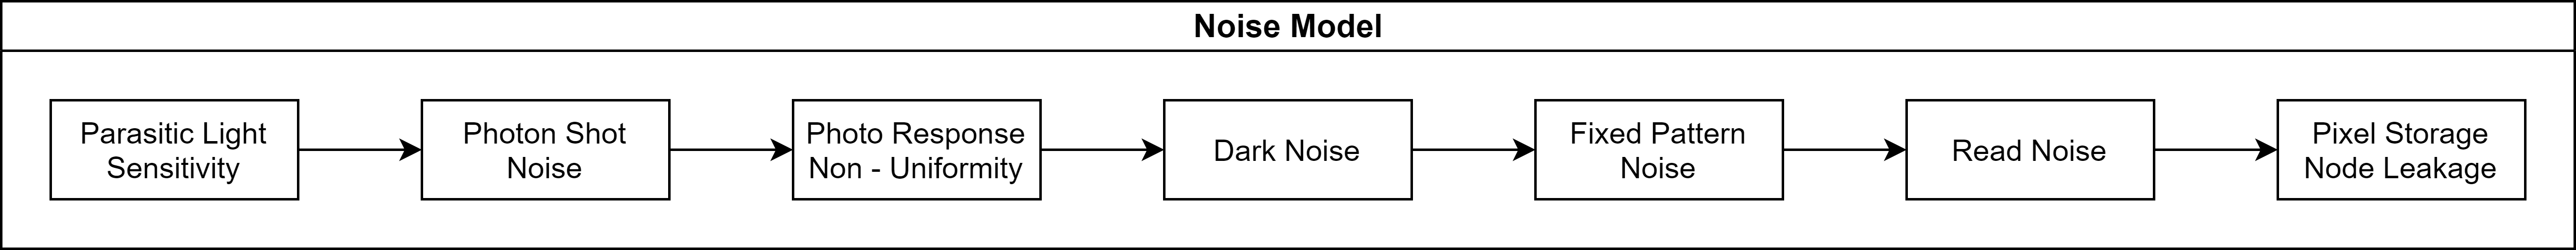
\includegraphics[scale=0.09]{Figures/Model/Noise Model.png}
    \caption{Noise Model - Version 2}
    \label{fig:SIS_v2_NM}
\end{Flowchart}

There are several image sensor noise sources that must be simulated in the camera model. Our image sensor of choice is a CMOS sensor, and so, we have focused on the noises specific to a CMOS Sensor. The noises that have been considered in the Sensor Model, in a chronological order are - \emph{Parasitic Light Sensitivity, Photon Shot Noise, Photo-Response Non-Uniformity, Dark Noise, Fixed Pattern Noise, Read Noise,} and \emph{Pixel Storage Node Leakage}.

The order is based on the following information - 
The photons are quantum particles, due to which, their detection at the CMOS Sensor follows Poisson Distribution, captured by the Photon Shot Noise. Photon Shot Noise, along with Parasitic Light Sensitivity, and the PRNU, are dependent on the inputs; so they are taken in the beginning. Dark Noise, Fixed Pattern Noise, Read Noise are independent of the input. Also, Pixel Storage Node Leakage needs to go to the last, because it refers to the number of pixels that leak out of the Storage Node.

% --- %
% PLS %
% --- %
\newpage

\subsubsection{Parasitic Light Sensitivity} % ???
\begin{wrapfigure}{r}{0.5\textwidth}
  \begin{center}
    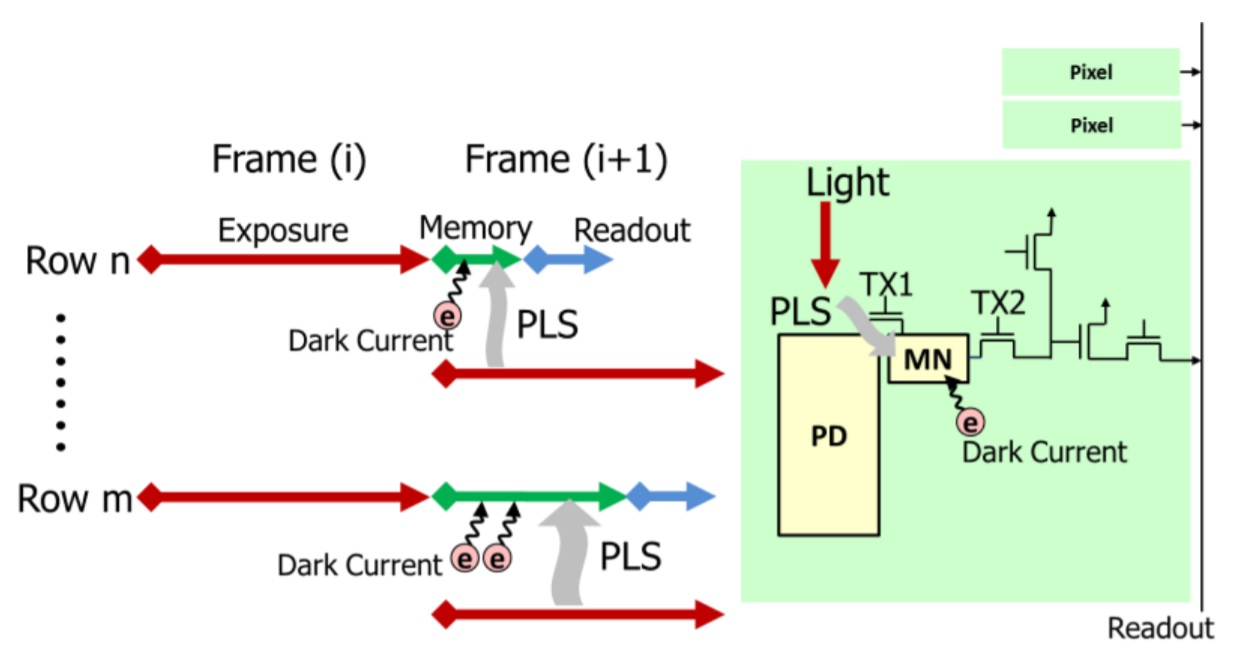
\includegraphics[width=0.48\textwidth]{Figures/Model/CMOS_PLS.jpeg}
  \end{center}
  \label{fig:PLS}
  \caption{Reading Method of Global Shutter Pixel}
\end{wrapfigure}

The adjoining figure shows a simple configuration and reading method of GS pixel. In order to realize \emph{Global Shutter (GS)} capability, a \emph{Memory Mode (MN)} must be added in each pixel . The electrons stored in the \emph{Photo Diode (PD)} are collectively read out to Memory Node and used as an image signal. The exposure is performed at once, but the readout is performed for each row as shown in the figure. Therefore, the electrons are generated in the Memory Node before the readout becomes noise, and leads to deterioration in image quality. When an image is output with much noise, the part of the picture that is read later becomes brighter or noisy because the noise is increased in later read rows. Accordingly, it is necessary to reduce the noise generated in the Memory Node. Major causes of the noise are light penetration into Memory Node and dark current.

PLS Noise is generated by light incident into Memory Node. An increase of PLS Noise leads to deterioration of image quality. This is because the charges generated by incident light to Memory Node are added to the charges stored in Memory Node after the exposure.

In dual transfer Global Shutter pixels, the photo-generated charges are transferred to MN. This allows a correlated double sampling (CDS) on a floating diffusion in successive transfer, which can reduce pixel noise to below 1 to 2 electrons.

\begin{equation*}
    \texttt{PLS} = \frac{\text{Photodiode Responsivity}}{\text{Storage Node Responsivity}} \quad (\text{Unitless Ratio})
\end{equation*}

The Memory Node is about 80,000x more sensitive than the Photodiode. However, the Memory Node is susceptible to photons only after the Shutter closes. So, the time to be taken into account is $(t_{Readout} - t_{Close})$. \newline

Formula Used in the code:
\begin{equation}
    \begin{aligned}
        \boxed{ \color{blue} PV =  PV_0 \cdot \left( 1 + \frac{1}{\texttt{PLS}} \cdot \left(\frac{t_{Readout} - t_{Close}}{t_{Capture}}\right) \right) \color{black}} 
    \end{aligned}
\end{equation}
where, $PV_0$ is the Pixel Value before \texttt{PLS} is applied, and $PV$ is the new Pixel Value. 

Note that the PLS Noise depends on the input illumination on the Sensor.

% Derivation:
% \begin{equation*}
%     \begin{aligned}
%         P_0 - \text{\# photons in } t_{Capture} & \rightarrow P_0 \\
%         P - \text{ \# photons in } (t_{Readout} - t_{Close}) & \rightarrow P_0 \cdot \left(\frac{t_{Readout} - t_{Close}}{t_{Capture}}\right) \\
%         \text{PV due to } P_0 \text{ in } t_{Capture} & \rightarrow PV_0 \\
%         \text{PV due to } P \text{ in } (t_{Readout} - t_{Close}) & \rightarrow \frac{PV_0}{PLS} \cdot \left(\frac{t_{Readout} - t_{Close}}{t_{Capture}}\right)
%     \end{aligned}
% \end{equation*}
% where, $PV$ is the Pixel Value. 



% --- %
% PSN %
% --- %
\newpage
\subsubsection{Photon Shot Noise} % 3.
\emph{Photon Shot Noise} (PSN), or \emph{Poisson Noise} refers to the inherent variation in the incident photon flux. Photoelectrons collected by a CMOS Sensor or a CCD Sensor exhibit a Poisson Distribution. (\cite{DSLRs}, \cite{Hasinoff2014})

Photons are discrete and the probability of one photon's arrival is independent of any other photon's arrival; so, individual photons detections can be treated as independent events that follow a random temporal distribution. Hence, the detection of photons at the sensor is a classical  \emph{Poisson Process}. 

Even from Quantum Statistics, a Poisson Distribution is obtained when photons are collected from an unvarying source over a set amount of time, which starlight effectively is, over the exposure time. 

Since the Poisson distribution approaches a normal distribution for large numbers, the photon noise in a signal will approach a normal distribution for large numbers of photons collected. However, instead of using a normal distribution, we stick to the Poisson Distribution as for the case of the CMOS Sensor for Star Tracker, the intensity of illumination at the Image Sensor can be low, where the Poisson Statistics are not reflected by a normal distribution. Hence, if the mean value of the number of photons that hit the sensor is $n$, the variance in the number of photons is the $\sqrt{n}$. 

\begin{wrapfigure}{r}{0.42\textwidth}
  \begin{center}
    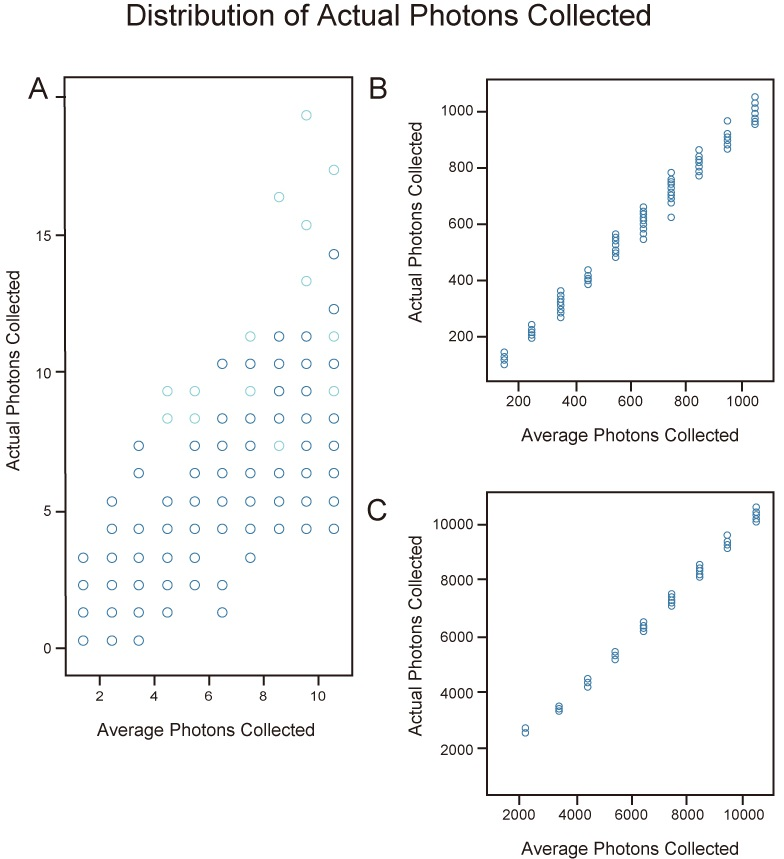
\includegraphics[width=0.4\textwidth]{Figures/Model/PSN_Hamamatsu.jpg}
  \end{center}
  \caption{(A) At low light levels, the variance introduced by photon shot noise contributes to a large proportion of the signal. (B, C) At higher light ranges, the variance introduced by photon shot noise is a smaller percentage of the overall signal. \cite{WhatIsPSN?}}
\end{wrapfigure}

The noise is therefore directly dependent on number of photons incident on the sensor. A very bright feature emitting many photons will have little (relative) noise. A very dim feature will look "granular", revealing that not many photons were averaged during its acquisition. This can not be known in advance just by looking at an empty calibration image. 

Moreover, Photon Shot Noise is not something intrinsic to the device but something in the nature of the photons that are averaged. Therefore it also depends on the acquisition time: the larger the exposure, the larger is the amount of photons gathered and the lesser the noise.

Hence, we use Random Numbers from Poisson Distribution. This is captured by the MATLAB function \texttt{poissrnd}, with the argument as the averaged number of photons, which is given by the number of photons incident in the no-noise case. 

The formula used in the code is:
\begin{equation}
    \boxed{ \color{blue} P = \texttt{poissrnd}(P_0) \color{black}}
\end{equation}

% ---- %
% PRNU %
% ---- %
\newpage
\subsubsection{Photo-Response Non-Uniformity} % 4.
When uniform light falls on a camera sensor, each pixel should output exactly the same value. However, small variations in cell size and substrate material result in slightly different output values. The difference between the true response from a sensor and a uniform response is known as \emph{Photo Response Non Uniformity} (PRNU).

Since PRNU is caused by the physical properties of the sensor itself, it is almost impossible to eliminate completely and is usually considered to be a normal characteristic of the sensor. It is a light sensitive noise and hence, signal-dependent.

PRNU in \% of Signal is the non-uniformity in spatial variation of pixel value for specific illumination.

The formula used in the code is:
\begin{equation}
    \boxed{ \color{blue} PV = PV_0 + \mathcal{N}(\texttt{PRNU} \cdot PV_0, \texttt{PRNU} \cdot PV_0)   \color{black}}
\end{equation}

where, $PV$ is the new Pixel Value, $PV_0$ is the old Pixel Value, \texttt{PRNU} is the PRNU Noise value in \%, and $\mathcal{N}(\mu, \sigma)$ is the Normal Distribution Function.

A Pseudo-Random Generator with a Seed Value is used to ensure that the noise remains same across iterations because \texttt{PRNU} Value is remains same for each pixel over time. 

% -- %
% DN %
% -- %

\subsubsection{Dark Noise} % 6. Dark Current, DSNU, Dark Noise
Dark Noise, given in no. of Electrons, is the noise due the reverse bias leakage current in all diodes. The average dark signal delivered by a sensor or a camera will be composed out of - a fixed DC offset, very often introduced by the analog circuitry on pixel/column/chip-level, or by an
extra black level offset, and a thermal component, also known as the dark current or leakage current. This part has a linear dependency on the exposure or integration time as well as temperature (at least if saturation of the sensor is not reached). The dark current decreases with decreasing temperature.

The Dark Temporal Noise is given in number of electrons and the Dark Signal / Dark Current is given in number of electrons per second. The variance of the Dark Noise is given as $DS \cdot t_S$.

As the dark current results from spontaneously generated electrons, the dark current is measured by simply "counting" these electrons. Since counting electrons obeys Poisson statistics, the noise associated with the dark current I is proportional to the square root of the number of dark electrons that accumulate during the exposure. 

Formula Used In the code:  
\begin{equation}
    \boxed{ \color{blue} PV = PV_0 + \texttt{G} \cdot \texttt{round}(\mathcal{N}(\texttt{DTN} + \texttt{DS} \cdot t_S, \sqrt{\texttt{DS} \cdot t_S}))   \color{black}}
\end{equation}

where, $G$ is the Gain, $PV$ is the new Pixel Value, $PV_0$ is the old Pixel Value, \texttt{DTN} is the Dark Temporal Noise value in \# $e^-$, \texttt{DS} is the Dark Signal in \# $e^-/s$, $t_S$ is the exposure time and $\mathcal{N}(\mu, \sigma)$ is the Normal Distribution Function.

Note that the rounding is important as number of electrons can't be a fractional number. 

% --- %
% FPN %
% --- %

\subsubsection{Fixed Pattern Noise} % 5.
FPN (also called non-uniformity) in LSB10 is the spatial percentage variation in pixel output values under uniform illumination due to device and interconnect parameter variations (mismatches) across the sensor. It is fixed for a given sensor, but can vary from sensor to sensor.This is the standard deviation value.

Fixed Pattern Noise is the variation in pixel dark signal over a frame and is determined by calculating Standard Deviation of mean image obtained from set of frame taken in dark.

Fixed Pixel Noise in LSB10 is the non-uniformity in spatial \% variation of
Pixel Values, independent of Specific Illumination.

This is the standard deviation value.

The formula used in the code is:
\begin{equation}
    \boxed{ \color{blue} PV = PV_0 + \mathcal{N}(0, \texttt{FPN})   \color{black}}
\end{equation}

where, $G$ is the Gain, $PV$ is the new Pixel Value, $PV_0$ is the old Pixel Value, \texttt{FPN} is the FPN noise value in LSB10, and $\mathcal{N}(\mu, \sigma)$ is the Normal Distribution Function.

A Pseudo-Random Generator with a Seed Value is used to ensure that the noise remains same across iterations because FPN Value is remains same for each pixel over time.

% -- %
% RN %
% -- %

\subsubsection{Read Noise} % 9.
Read noise is a combination of noise from the pixel and from the ADC. The Read Noise (RN) of the sensor is the equivalent noise level (in electrons RMS) at the output of the camera in the dark and at zero integration time. The ADCs for a CMOS image sensor are present for each pixel.

Read noise basically determines the contrast resolution that the camera is able to achieve. The lower the read noise level, the lower the minimum number of signal electrons that can be detected. Read noise is also important in combination with expressing the sensitivity of a camera. 

It is one of the main sources of noise in an imaging camera for relatively short exposures. Low read noise is desirable as it allows the camera to detect low level signals and attain a high dynamic range and therefore results in a more sensitive sensor.

The read noise of the CMOS sensor is a noise distribution and is normally given as in $e^-$, as a median value.

Formula used in the code:
\begin{equation}
    \boxed{ \color{blue} \texttt{DNR} = 20 \cdot \log_{10} \left(\frac{\texttt{FWC}}{\texttt{Read Noise}} \right) \color{black} }
\end{equation}

where, \texttt{DNR} is the Dynamic Range of the Pixel, \texttt{FWC} is the Full Well Count. 

Note that the Read Noise is an almost constant value.

% ---- %
% PSNL %
% ---- %

\subsubsection{Pixel Storage Node Leakage} % 7. 

In a global shutter, after exposure the integrated charge from each pixel is transferred to the pixel storage node. Since this is typically diffusion, it has some leakage. The storage nodes of some pixels are leakier than others, resulting in the bright spots that can be seen in images with larger frame times and the default timing.

The storage node of each row is reset during the row overhead time of the previous frame. The time between 2 resets of the floating diffusion is therefore equal to $\frac{1}{frame rate}$.

Formula Used in the code:
\begin{equation}
    \boxed{ \color{blue} PV = PV_0 - \texttt{G} \cdot \texttt{round}(\texttt{PSNL} \cdot (t_{Readout} - t_{Close}) \color{black}}
\end{equation}

where, $G$ is the Gain, $PV$ is the new Pixel Value, $PV_0$ is the old Pixel Value, \texttt{PSNL} is the PSNL noise value in \# electrons.


 
% ------------- %
% Sample Images %
% ------------- %
 
\subsubsection{Sample Images}
These are some images generated using the \SISM Version 2 in Figure \ref{fig:sample_images}.

\begin{figure}[h!]
    \centering
    \begin{subfigure}[b]{0.45\textwidth}
        \centering
        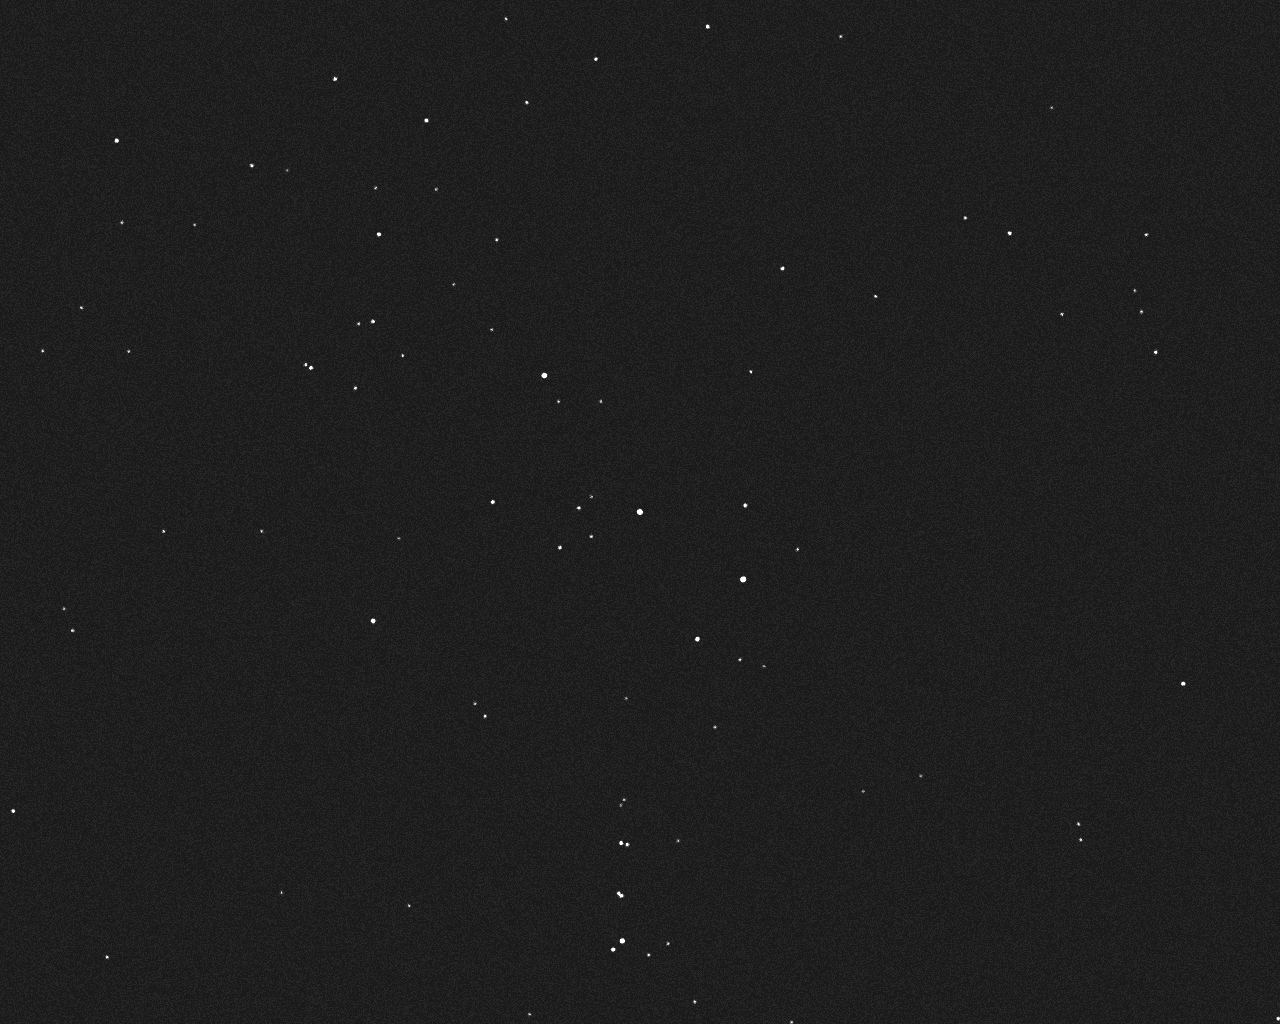
\includegraphics[width=\textwidth]{Figures/Model/Sample Images/Image_1.png}
        \caption{Sample Image 1}
        \label{fig:sample_1}
    \end{subfigure}
    \hfill
    \begin{subfigure}[b]{0.45\textwidth}
        \centering
        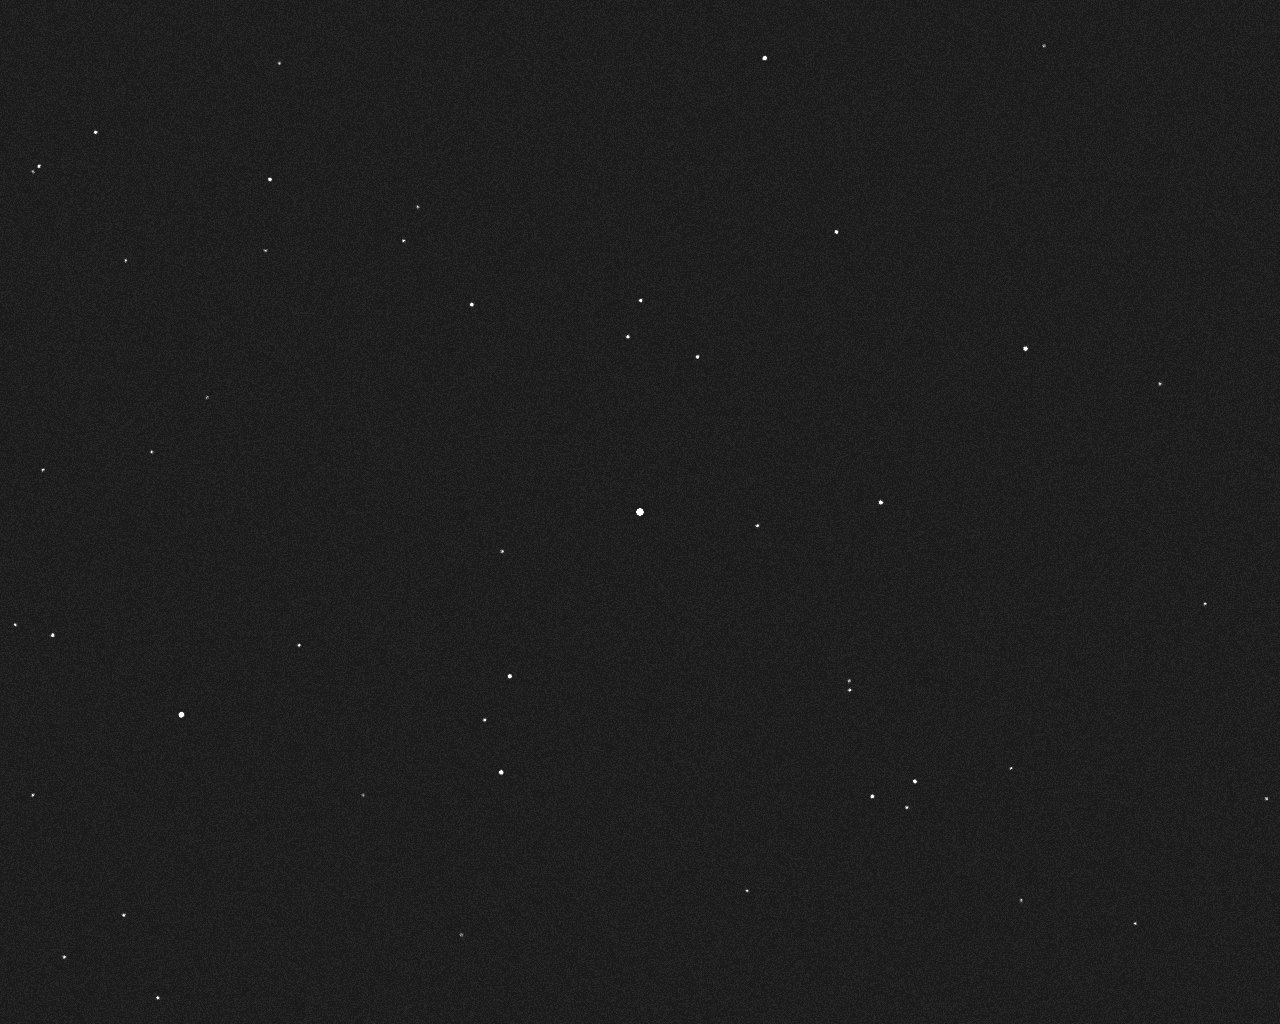
\includegraphics[width=\textwidth]{Figures/Model/Sample Images/Image_2.png}
        \caption{Sample Image 2}
        \label{fig:sample_2}
    \end{subfigure}
    \\
    \begin{subfigure}[b]{0.45\textwidth}
        \centering
        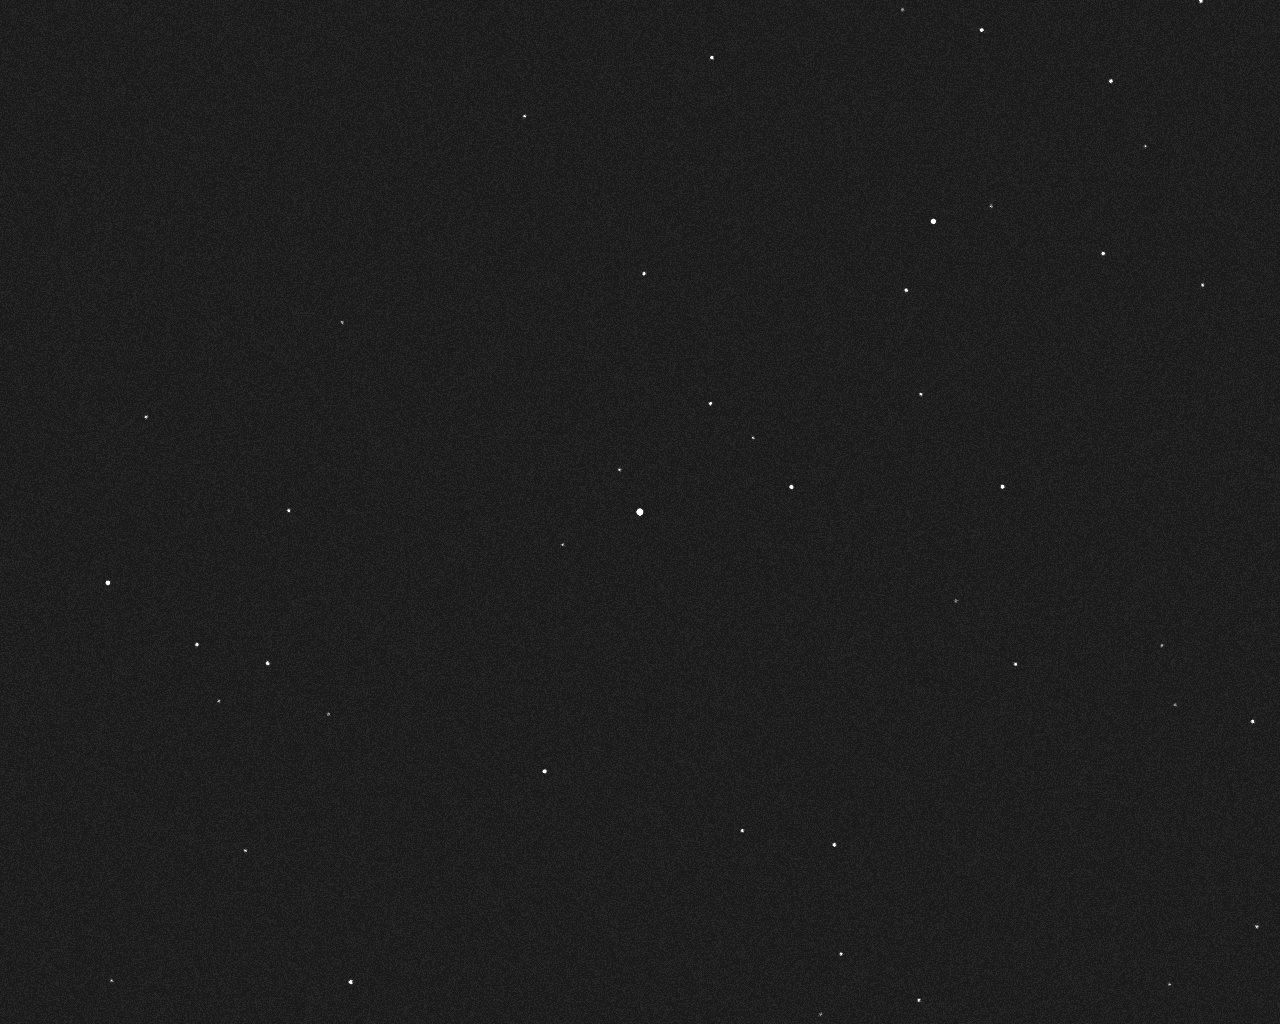
\includegraphics[width=\textwidth]{Figures/Model/Sample Images/Image_3.png}
        \caption{Sample Image 3}
        \label{fig:sample_3}
    \end{subfigure}
    \hfill
    \begin{subfigure}[b]{0.45\textwidth}
         \centering
         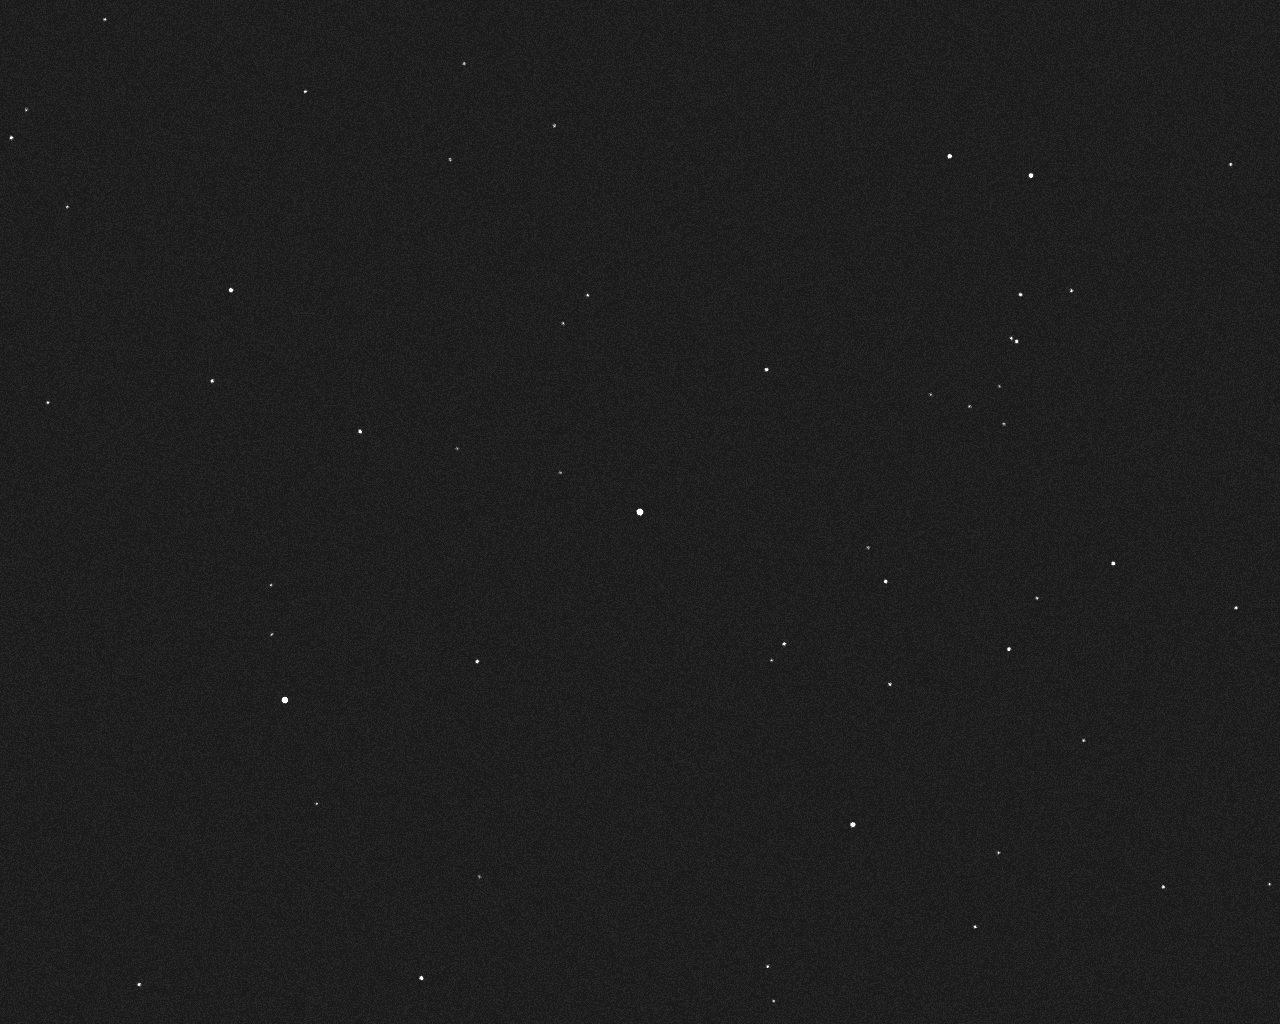
\includegraphics[width=\textwidth]{Figures/Model/Sample Images/Image_4.png}
         \caption{Sample Image 4}
         \label{fig:sample_4}
    \end{subfigure}
    \\
    \begin{subfigure}[b]{0.45\textwidth}
        \centering
        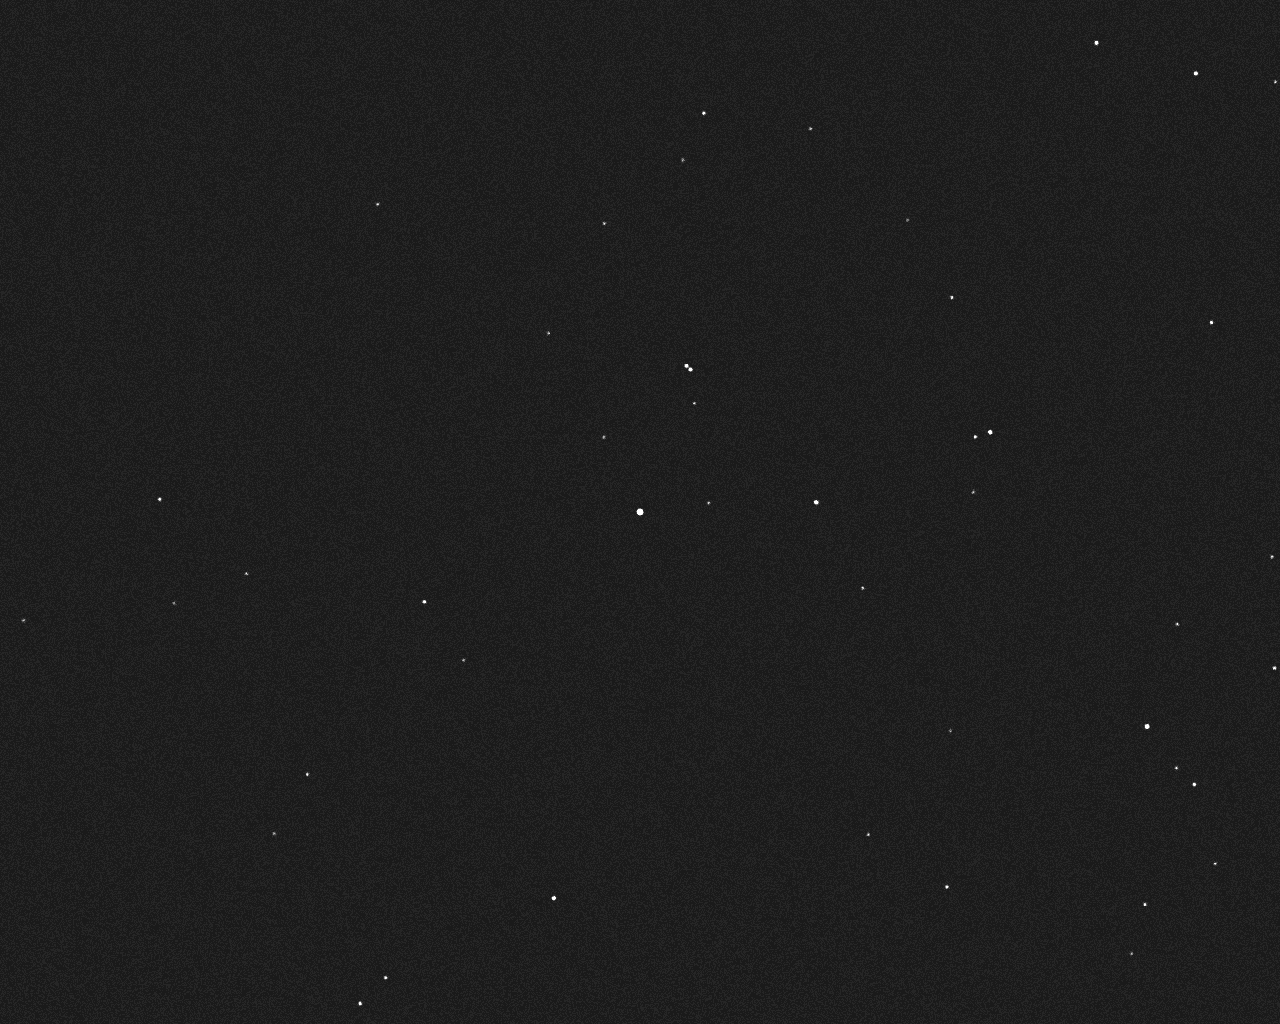
\includegraphics[width=\textwidth]{Figures/Model/Sample Images/Image_5.png}
        \caption{Sample Image 5}
        \label{fig:sample_5}
    \end{subfigure}
    \hfill
    \begin{subfigure}[b]{0.45\textwidth}
         \centering
         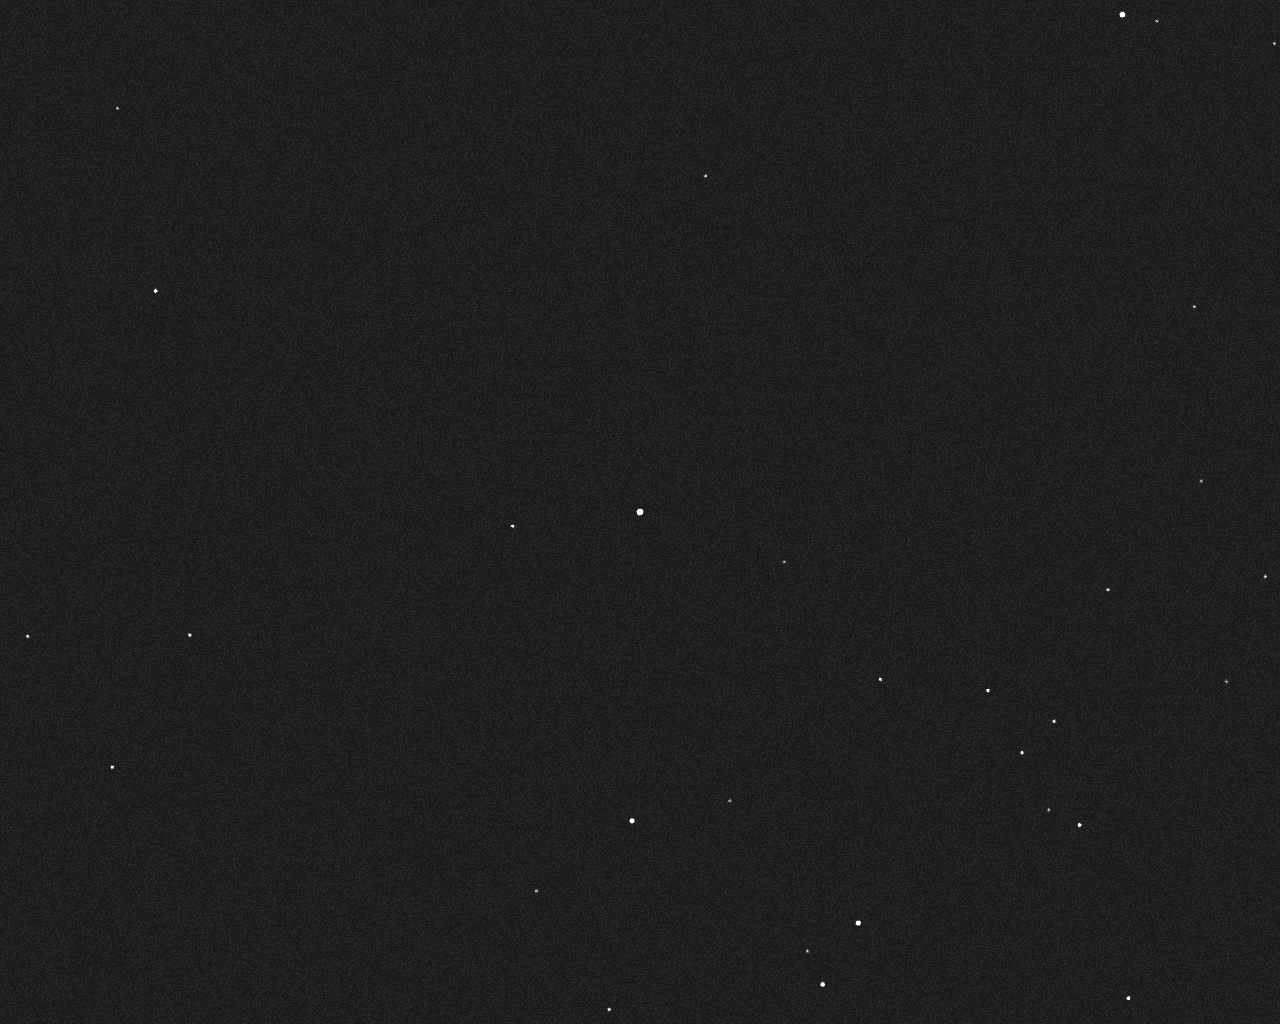
\includegraphics[width=\textwidth]{Figures/Model/Sample Images/Image_6.png}
         \caption{Sample Image 6}
         \label{fig:sample_6}
    \end{subfigure}
    \caption{Sample Images}
    \label{fig:sample_images}
\end{figure}


\end{document}